\documentclass[10pt, conference, compsocconf, twocolumn]{IEEEtran}
%
%\usepackage{latex8}
\usepackage{times}
\usepackage{graphicx}
\usepackage{setspace}
\usepackage{algorithmic}
\usepackage{algorithm}
\usepackage{epstopdf}
\DeclareGraphicsExtensions{.pdf,.png,.jpg,.bmp,.eps}
\setstretch{1.01}

\def\dijkstra{%
    \REQUIRE $nodes.length() \geq 1$
    \STATE $openNodeList \Leftarrow new List$
    \STATE $openNodeList.add(0)$
    \WHILE{ $openNodeList.size() \neq 0$}
        \STATE $curNode \Leftarrow ClosestNode$
        \FOR{$i = 1$ to $nodes.length()$}
            \IF{$nodes[i] \neq Finalized$}
                \IF{$NodesWithinRange(curNode,i) = $ true}
                    \IF{ $openNodeList.contains(i) \ne$ true}
                        \STATE $nodes[i].Head \Leftarrow curNode$
                        \STATE $openNodeList.add(i)$
                    \ENDIF
                \ENDIF
            \ENDIF
        \ENDFOR
        \STATE $nodes[curNode] \Leftarrow Finalized$
        \STATE $openNodeList.remove(curNode)$
    \ENDWHILE
}

\def\checkDetection{%
    \FOR{$i = 1$ to $nodes.length()$}
        \IF{$Intruder Within Range$}
            \STATE $sendToBase()$
        \ENDIF
    \ENDFOR
}

\def\BaseRecieveDetection{%
    \REQUIRE $node \neq null \vee curNode \geq 0$
    \IF{$node.distanceToBase > 0$}
        \IF{$SensingType = SINGLEDETECTION$}
            \STATE{$Detected = true$}
        \ELSE
            \STATE{$nodesWithDetect[curNode] \Leftarrow  node$}
            \STATE{$curNode \Leftarrow curNode + 1$}
        \ENDIF

    \ENDIF
}

\def\BaseUpdate{%
    \REQUIRE $SensingType \neq null \vee GlobalVars \neq null$
    \IF{$SensingType = ThreeIndividual$}
        \IF{$detections \geq GlobalVars.getK()$}
            \STATE{$Detection \Leftarrow  true$}
        \ENDIF
    \ELSE
        \IF{$SensingType = ThreeSimultaneous$}
            \IF{$curNode \geq GlobalVars.getK()$}
                \STATE{$tmpDetection \gets CountNumDetections()$}
            \ENDIF
            \IF{$tmpDetections \geq GlobalVars.getK()$}
                \STATE{$Detection \Leftarrow true$}
            \ENDIF
        \ENDIF
    \ENDIF
}

 \ifCLASSINFOpdf \else \fi

\hyphenation{op-tical net-works semi-conduc-tor}

\begin{document}
\title{Joint and Simultaneous $K$-sensor Detection in Deterministic and Random Sensor Networks}
%\title{A Novel Mobility Model for Analyzing Intrusion Detection in Wireless Sensor Networks}

\author{\IEEEauthorblockN{Yun Wang, Andrew Kutta}
\IEEEauthorblockA{Department of Computer Science\\
Southern Illinois University Edwardsville\\
Illinois, USA\\
Email: yuwang@siue.edu, akutta@siue.edu}}
\maketitle


\begin{abstract}

\end{abstract}

\begin{IEEEkeywords}
Intrusion detection; Intrusion path; Network deployment; Sensing
range; Wireless sensor networks; \\
\end{IEEEkeywords}

\IEEEpeerreviewmaketitle

\section{Introduction}

\begin{figure} [b]
  % Requires \usepackage{graphicx}
  \centering
  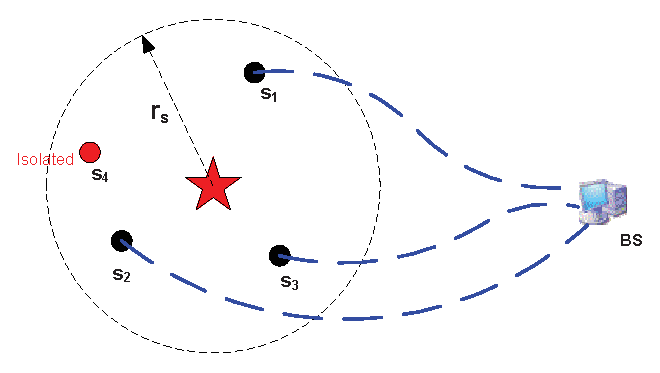
\includegraphics[width=2.8 in]{SimultaneousKDetection.eps}\\
  \caption{An instance of Simultaneous $K$-sensor detection of a static/mobile object}\label{SimultaneousKDetection.eps}
\end{figure}
\begin{figure} [t]
  % Requires \usepackage{graphicx}
  \centering
  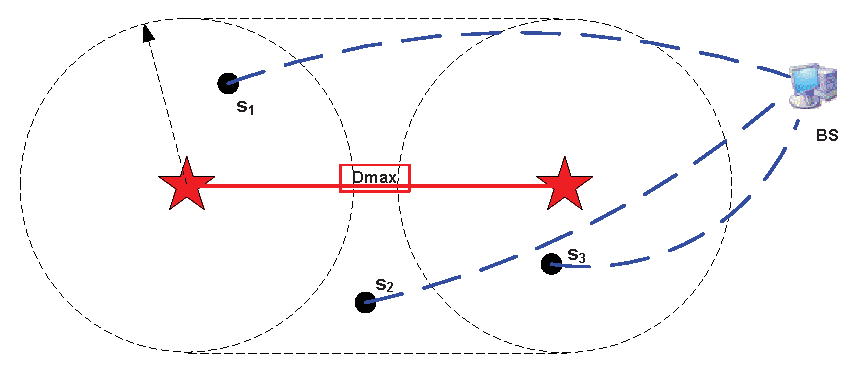
\includegraphics[width=3.2 in]{JointKDetection.eps}\\
  \caption{An instance of Jointly $K$-sensor detection of a mobile object}\label{JointKDetection.eps}
\end{figure}




Wireless Sensor Networks (WSNs) are deployed for a broad range of
civil or military applications to serve various purposes under
different requirements. As an example, some application requires an
object being detected by at least $k$ sensors \emph{simultaneously}
to fulfill its task such as determining the object's location and
track its trajectory. This
\textbf{simultaneous-$k$-sensing-detection} is of paramount
importance to some WSN applications [reference]. Fig.
\ref{SimultaneousKDetection.eps} illustrates an instance of
\emph{simultaneous }$K$-sensor detection of an object. In the
depicted scenario, sensors $s_1$, $s_2$, $s_3$ and $s_4$ can
simultaneously detect the object but only $s_1$, $s_2$ and $s_3$ can
send the sensing data to the base station(BS) as they are connected
with the BS while sensor $s_4$'s detection does not contribute to
the simultaneous-$k$-sensing-detection as it is isolated from the
BS.  In other words, the scenario shown in Fig.
\ref{SimultaneousKDetection.eps} only satisfies the requirements of
simultaneous-$3$-sensing-detection.

In fact, $k$-sensing detection is not a brand new concept and has
been discussed extensively in the literature. However, most of the
research work are focus on \textbf{joint-$k$-sensing-detection}, in
which an mobile object can be detected by the WSN as long as at
least $k$ sensors can detect it within application-specified time or
distance. Fig. \ref{JointKDetection.eps} illustrates an instance of
joint-$k$-sensing-detection, in which $s_1$, $s_2$, and $s_3$ can
not detect the mobile object simultaneously, but they can jointly
detect it before the object travels a maximum allowable intrusion
distance of $D_{max}$ in the WSN.

To be completed by YW



% no \IEEEPARstart
%
%The remainder of this paper is organized as follows. Section
%\ref{sec:related_work} presents the related work. Section
%\ref{sec:network_model} presents the network model, intrusion model,
%and the evaluation metrics. Section
%\ref{sec:intr_detection_analysis} explores the relationships between
%the detection probability and the network configuration parameters.
%Section \ref{sec:simulation} demonstrates the theoretical and
%simulation results. Finally, this paper is concluded in section
%\ref{sec:conclusion}.\\
%

\section{Related Work} \label{sec:related_work}


\section{Intrusion Detection Network Model and Definitions}\label{sec:network_model}
Our network model includes a network model, a intrusion detection
model, and the performance evaluation metrics.
\subsection{Network Model} \label{sec:model_A}
We consider a homogeneous WSN in a two dimensional square plane with
an area of $A=L \times L$. A number of \emph{N} sensors, denoted by
a set \textbf{N} = ($n_1$, $n_2$, $...$ , $n_N$), are deployed in
$A$ following deterministic or random sensor deployment approach. In
random deployment, sensor are assumed to be uniformly and
independently following a two-dimensional Poisson point
distribution, and in random deployment, sensors are deployed
following a square or triangle pattern, as illustrated in Fig.
\ref{SquareTriRandomDeployment.eps}. In such a network model, all
sensors are assumed to be static once the WSN has been deployed and
all have the same sensing range of $r_s$ and a transmission range of
$r_c$.

\begin{figure}
  % Requires \usepackage{graphicx}
  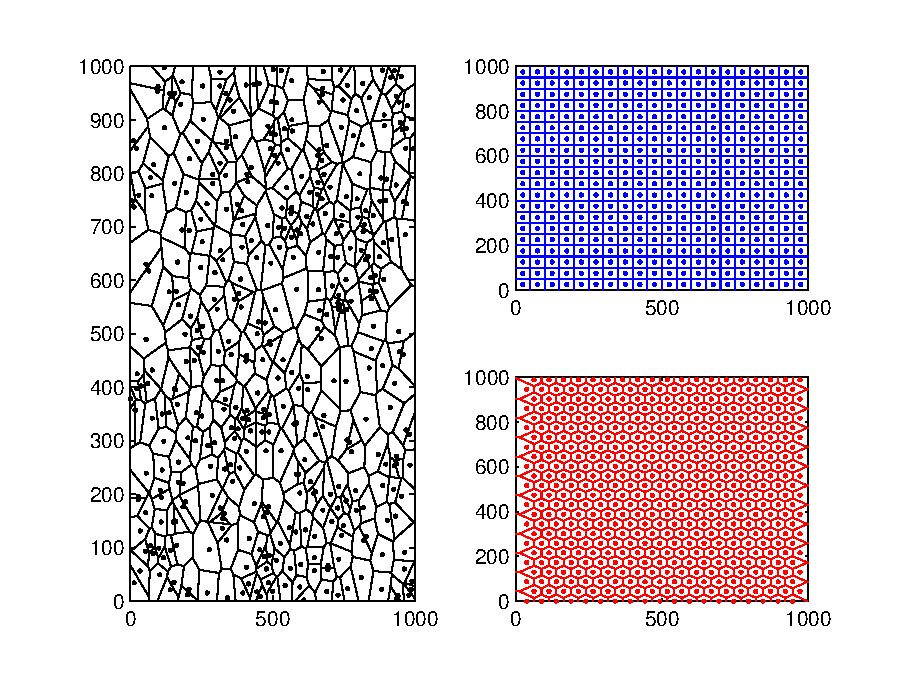
\includegraphics[width=3.2 in]{SquareTriRandomDeployment.eps}\\
  \caption{Random and Deterministic Sensor Deployment}\label{SquareTriRandomDeployment.eps}
\end{figure}


\subsection{Sensing and Detection Model}\label{sec:model_C}
\begin{itemize}
  \item \textbf{simultaneous-$k$-sensing-detection}: To be completed
  by YW
  \item \textbf{Joint-$k$-sensing-detection}: To be completed by YW
\end{itemize}





%
% should be determined from at least three sensors'
%sensing data. In view of this, we employ both single-sensing
%detection and multiple-sensing detection models in this work. In
%single-sensing detection, an intruder is detected if it enters into
%one of the sensor's sensing range. In $k$-sensing detection, at
%least $k$ sensors should collaborate to detect the intruder.  To
%extend upon the single-sensing detection model, a third model is
%used.  A successful detection occurs when an intruder enters $k$
%sensor's sensing range, regardless of the time delay since the $k-i$
%detection, where $0 < i < k$.


\subsection{Evaluation Metrics}
In order to evaluate the quality of intrusion detection in WSNs, we
use the metrics defined in \cite{Intru_TMC} as follows:
\begin{itemize}
  \item \textbf{Intrusion Distance}: The intrusion distance, denoted by
$D$, is the distance between the point where the intruder enters the
WSN and the point where the intruder gets detected by any sensor(s).
$\xi$ is the maximal distance allowable for the intruder to move
before it is detected by the WSN for an application.

%\item \textbf{Maximal Allowable
%Intrusion Distance}: Following the definition of intrusion distance,
%the Maximal Intrusion Distance (denoted by $\xi$, $\xi > 0$)  In
%other words, if the intruder is detected within $\xi$, the
%performance of the WSN is satisfiable, otherwise, the WSN needs
%reconfiguration.

  \item \textbf{Detection Probability}: The detection probability is defined as
the probability that an intruder is detected within the Maximal
Intrusion Distance, $\xi$)
 \item \textbf{Average Intrusion Distance}: The average intrusion distance is
defined as the expected distance that the intruder travels before it
is detected by the WSN for the first time.\\
\end{itemize}


\section{Analysis and Derivation}\label{sec:intr_detection_analysis}

To be completed by YW.



\section{Simulations}

\subsection{Design and Implementation}

%\textbf{Drew: 1) I will need you to work on this subsection; 2)
%Please read the attached paper "Robot World as a Teaching Aid for
%Object-Oriented Programming in Java" on sections 4 to 6 for
%reference; 3) please use Visio to draw diagrams of simulation
%architecture, and send me the vsd files; 4) Design and implement a
%GUI in which users can adjust the network parameters and see the
%corresponding intrusion distance and where it is detected.}
%
%I am working on the rest of this paper and will let you know if more
%results are needed.




Implemented are two different interfaces, a Graphical User Interface
and an Automated Driver.  The User Interface uses a single thread to
run a single iteration of the simulator with the user defined parameters.
The Automated Driver uses three threads to simulate Simultaneous K Detection,
Joint K Detection, and Single Detection Sensing Models.  Each detection type is
 tested with variable sensing and communication ranges averaged over a user defined number of
 iterations per range before incrementing either the communication or sensing range.

\begin{figure} [h]
  % Requires \usepackage{graphicx}
  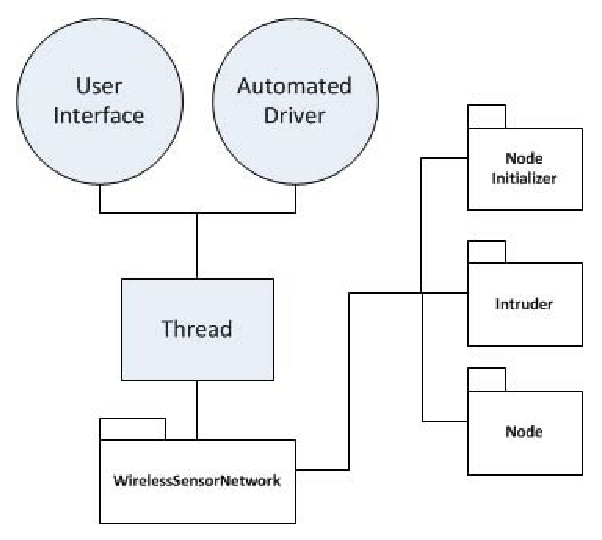
\includegraphics[width=3.2 in]{BasicArchitecture.eps}\\
  \caption{Generalized Architecture of the Simulator}\label{BasicArchitecture.eps}
\end{figure}

%\begin{figure} [h]
%  % Requires \usepackage{graphicx}
%  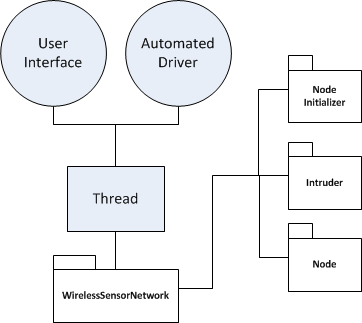
\includegraphics[width=3.2 in]{BasicArchitecture.png}\\
%  \caption{Generalized Architecture of the Simulator}\label{BasicArchitecture.png}
%\end{figure}

The WSN simulator includes three packages: Node, Intruder, and Node
Initializer. The Node Initializer is used to place the Nodes
according to the selected distribution pattern such as random,
square, or triangle. The Intruder is called by the WSN to update
it's position at every tick, once updated the WSN package iterates
through all Nodes to determine if the Intruder is within the sensing
range.  A sub-package of Node is the Base Station (BS). The BS
handles all detections and filters out invalid detections due to not
meeting detection type or due to lack of connectivity.

 \begin{figure} [h]
  % Requires \usepackage{graphicx}
  \centering
  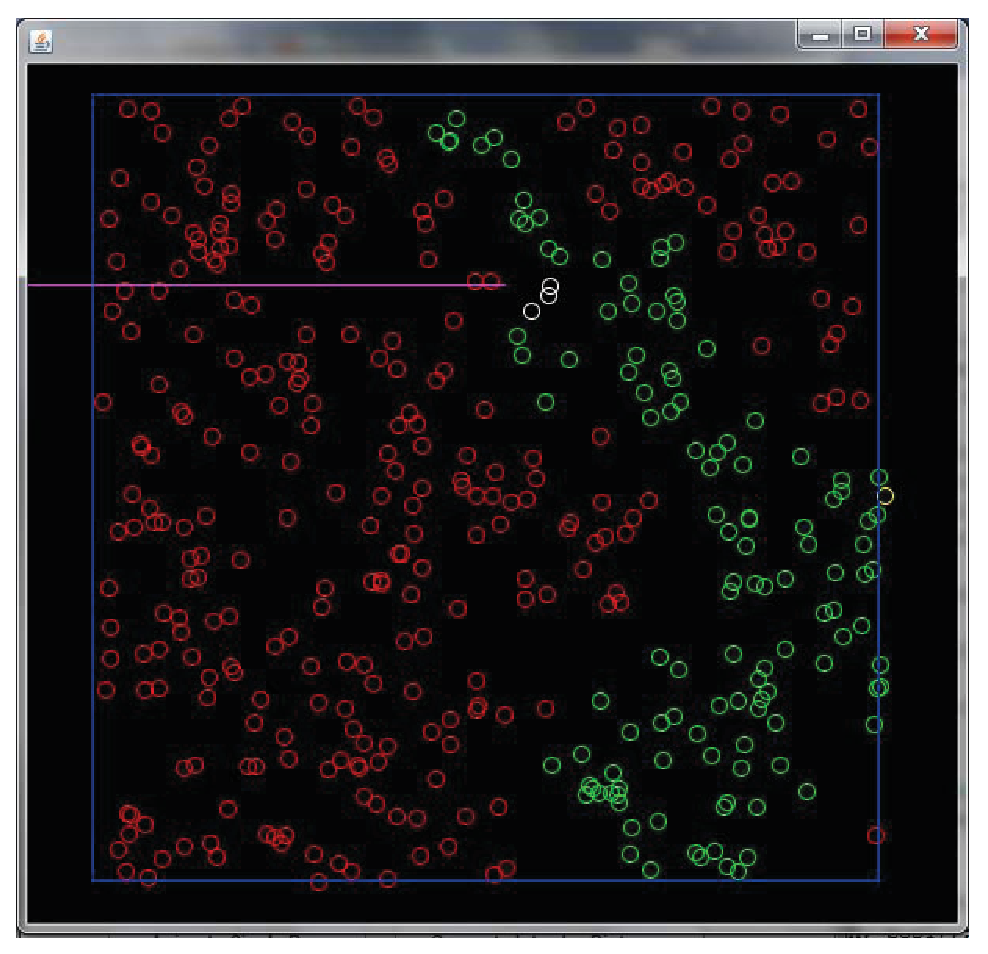
\includegraphics[width=1.6 in]{SingleAnimationExample2.eps}\\
  \caption{Example Iteration with Communication Range equal to $70$}\label{SingleAnimationExample2.eps}
\end{figure}

The Graphical User Interface can be used to demonstrate a single
iteration with the user defined parameters, or run a variable amount
of iterations with the parameters.  As illustrated in
\ref{SingleAnimationExample2.eps}, with random distribution it is
possible to have many of the nodes that would normally be fully
connected be sectioned off and non-viable for detecting intruders.


The second functionality of the GUI is to compute the average
distance traveled by an intruder.  This interface is shown in Fig.
\ref{AvgIntruderDistanceAverage.eps}. It roots more into the
automated driver method by creating a thread and performing up to
$1000$ iterations.

\begin{figure} [h]
  % Requires \usepackage{graphicx}
  \centering
  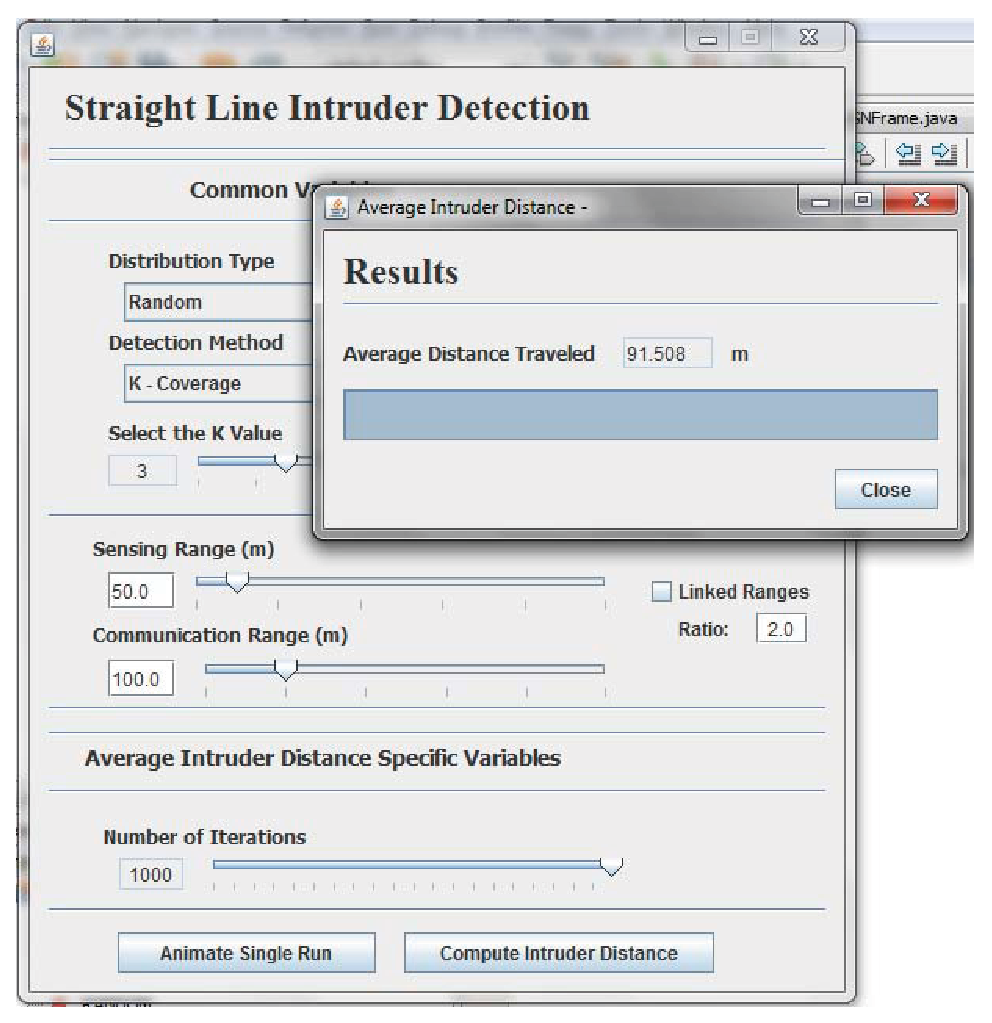
\includegraphics[width=2.5 in]{AvgIntruderDistanceAverage.eps}\\
  \caption{Interface when computing average intruder distance over $1000$ iterations}\label{AvgIntruderDistanceAverage.eps}
\end{figure}


\subsection{Results and Discussions}


For every Sensor Distribution Models used, the sensing range begins
at $27$ meters and is incremented by $2$ meters until a maximum of
$77$ meters is reached.  For each sensing range, the test was
averaged over $1000$ iterations in order to achieve a reliable
result.


In order to determine whether the intruder is detected, three
detection strategies are deployed.  These strategies will be
explained later in this section.  Each strategy relies on being
connected to a base station.  The sensor network is deployed over
a $1000$x$1000$ meter area with the base station statically located
at $1000$x$500$ in each deployment method.  General strategy used to determine
connectivity is the Dijkstra's Algorithm.  The version implemented is explained
below.

\begin{algorithm}
\caption{Dijkstra's Algorithm}
    \begin{algorithmic}
        \dijkstra
    \end{algorithmic}
\end{algorithm}

%\begin{figure}[h]
%\scalebox{0.4} {
%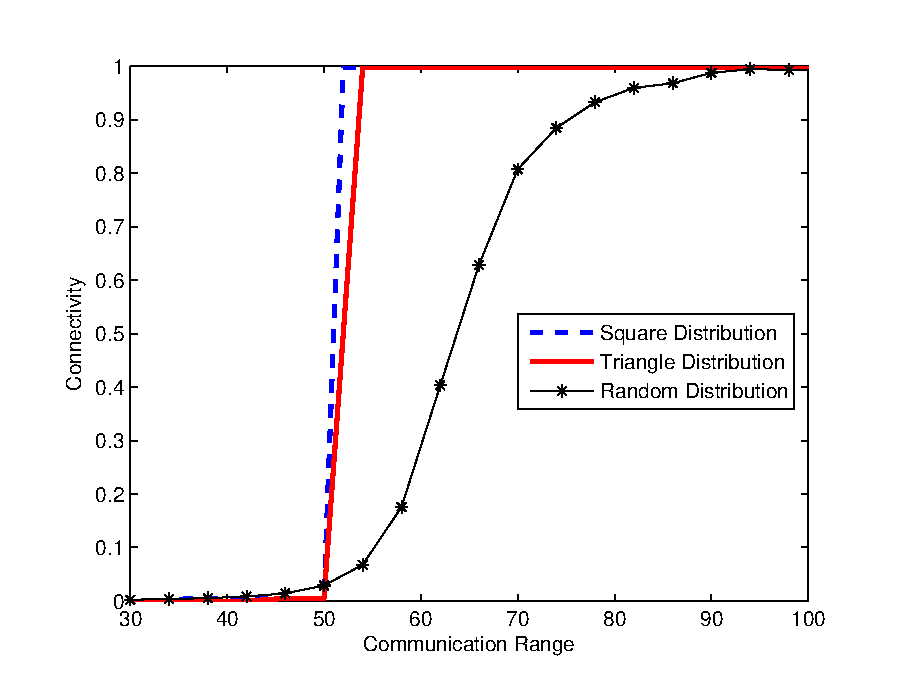
\includegraphics{connectivitySquareTriangleRandom.eps}}
%\begin{caption} {
%Connectivity of Sensors.  Communication range of sensors are $2 *$ Sensing Range.
%}
%\end{caption}
%\end{figure}


\begin{figure} [b]
  % Requires \usepackage{graphicx}
  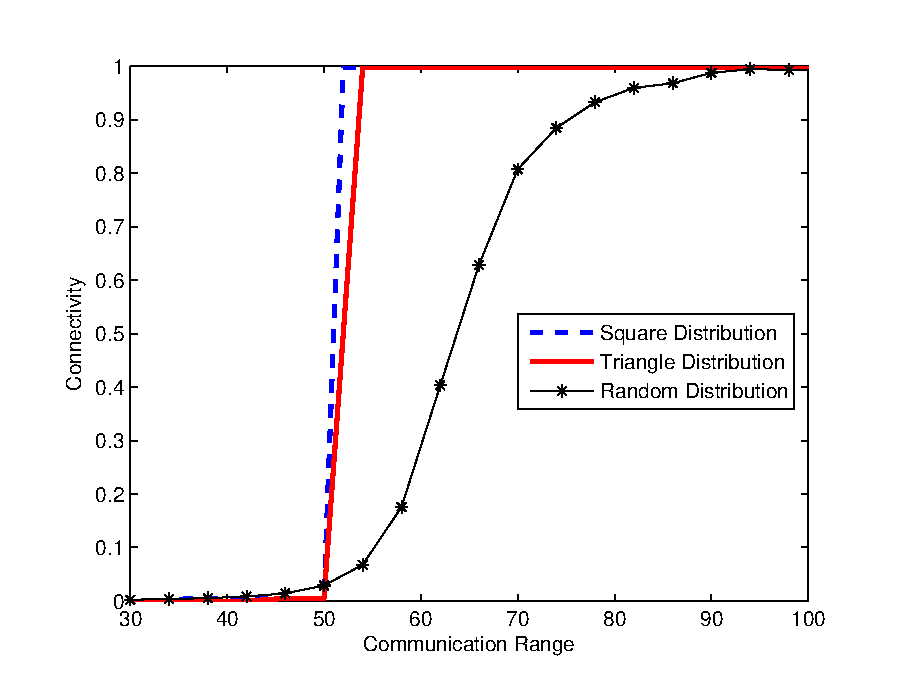
\includegraphics[width=3.2 in]{connectivitySquareTriangleRandom.eps}\\
  \caption{Connectivity of Sensors.  Communication range of sensors are $2 *$ Sensing Range}\label{connectivitySquareTriangleRandom.eps}
\end{figure}



\begin{figure}
\centering
  % Requires \usepackage{graphicx}
  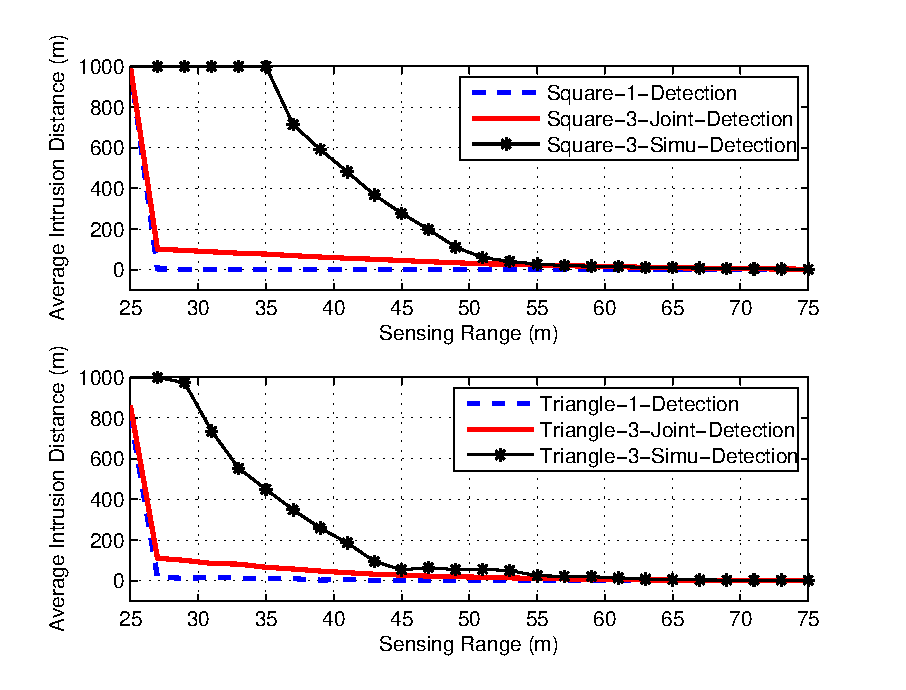
\includegraphics[width= 3.2 in]{AveIntruDistance_SquareTriangle.eps}\\
  \caption{Average Intrusion Distance in a lattice WSN following Square and Triangle Patterns}\label{AveIntruDistance_SquareTriangle.eps}
\end{figure}

\begin{figure}
\centering
  % Requires \usepackage{graphicx}
  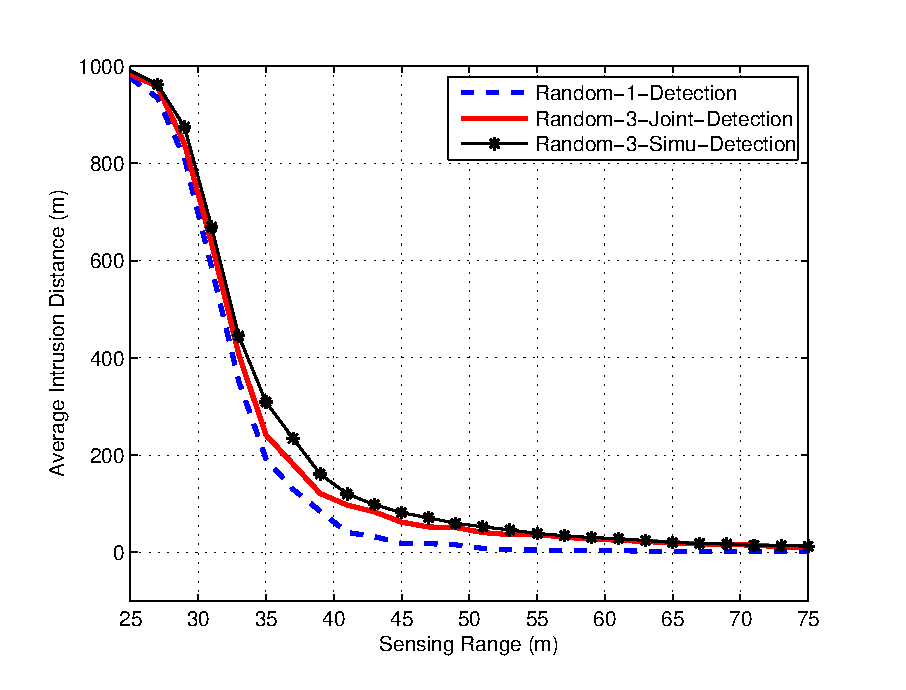
\includegraphics[width= 3.2 in]{AveIntruDistance_Random.eps}\\
  \caption{Average Intrusion Distance in a Random WSN}\label{AveIntruDistance_Random.eps}
\end{figure}


\begin{figure}
  % Requires \usepackage{graphicx}
  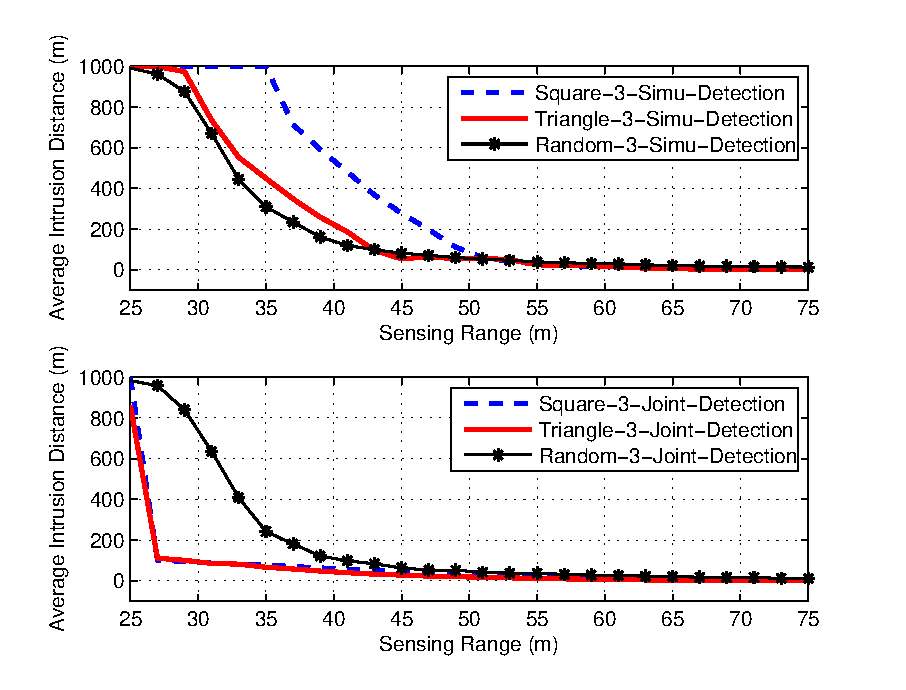
\includegraphics[width= 3.2 in]{AveIntruDistance_RanTriSquare_3_Simu_Joint.eps}\\
  \caption{Average Intrusion Distance in a Random WSN under $3$ jointly and Simultaneously Detection}\label{AveIntruDistance_RanTriSquare_3_Simu_Joint.eps}
\end{figure}

\begin{figure}
  % Requires \usepackage{graphicx}
  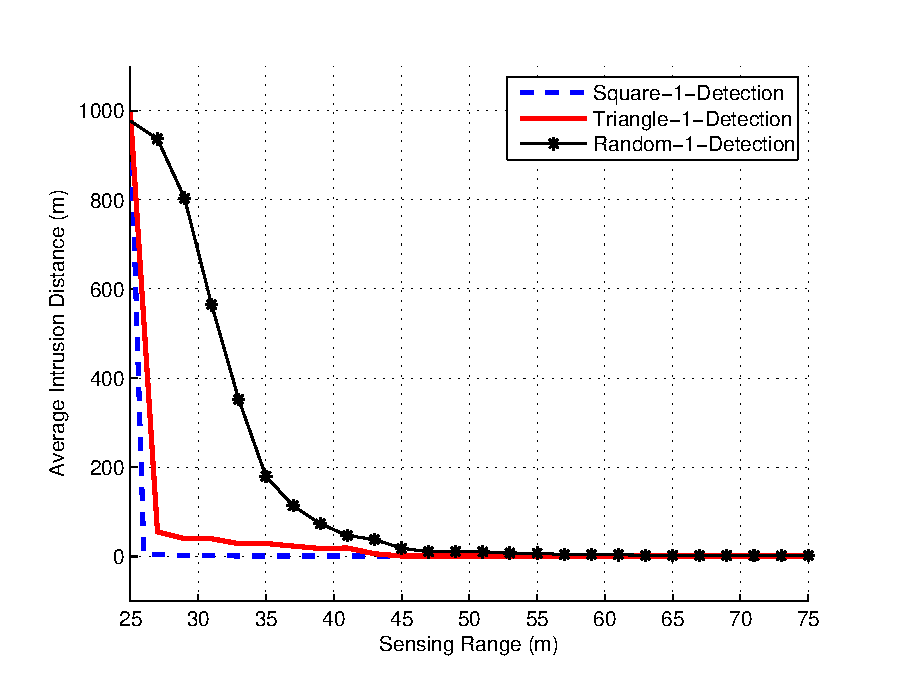
\includegraphics[width= 3.2 in]{AveIntruDistance_RanTriSquare_SingleDetection.eps}\\
  \caption{Average Intrusion Distance in a Random WSN under single-sensing detection}\label{AveIntruDistance_RanTriSquare_SingleDetection.eps}
\end{figure}



The Sensor Connectivity graph is the result of running Dijkstra's
Algorithm after each generation of the Sensor Network.  A generation
of the Sensor Network is considered a single iteration.  There are
$1000$ iterations performed per sensing range, or, in this case,
communication range.  The communication range is defined as twice
the sensing range.  It is easily seen that the limiting factor for
the random distribution is the connectivity of the network.
Although, initially the random distribution performs better.

In the simulator created, the universal update() call is sent to the
Wireless Sensor Network, which in turn requests that the intruder
updates as well.  When an intruder is updated, it's position is
updated based on it's own algorithm.  For the Straight-Line
Intruder, this means that the intruder moves one meter towards the
goal.  After the intruder is updated, the wireless sensor network
must check for a detection.  This is done using the below algorithms
where IntruderWithinRange is defined as the Euclidean Distance of
the intruder compared with the sensor.  The distance is then
compared with the sensor's sensing range.

\begin{algorithm}
\caption{Check For Detection}
    \begin{algorithmic}
        \checkDetection
    \end{algorithmic}
\end{algorithm}

At this point, if the sensor has detected an intruder, it sends that
information to the base station.  The information transfered to the
base is mainly the index of the current sensor within the array.

\begin{algorithm}
\caption{Base Recieve Detection}
    \begin{algorithmic}
        \BaseRecieveDetection
    \end{algorithmic}
\end{algorithm}

Once every node has been checked for a detected intruder, the base
station processes all of the potential detections.  At this point
the Base Recieve Detection algorithm is employed.  Before any
processing occurs, it checks to make sure that the detection is
valid.  It is only considered valid if the node is able to
communicate with the base station.  If the sensor cannot communicate
with the base, then the detection message is ignored.  Otherwise the
base station counts the detection and raises the Detected flag
depending on the sensing strategy being used.

\subsection{Single-sensing Detection}
%
%\begin{figure}[H]
%\scalebox{0.35}
%{ \includegraphics{singleDetectionProbability.jpg}}
%\begin{caption} {
%An intruder is considered detected when found by a single sensor that can communicate with the base.  In this case, the non-random distribution of sensors become very efficient when compared to the random distributions.
%}
%\end{caption}
%\end{figure}
%
%\begin{figure}[H]
%\scalebox{0.35}
%{ \includegraphics{singleDistanceTraveled.jpg}}
%\begin{caption} {
%This shows the average distance traveled at a variety of sensing ranges for the Square, Triangle, and Random Distributions.   There are 400 Nodes deployed using a single node detection strategy.
%}
%\end{caption}
%\end{figure}

The Single-Sense Detection Strategy will flag the intruder as
detected by any node that can communicate with the Base Station
which is located at $(1000,500)$ in the Sensor Network.  As can be
seen, as soon as the Square and Triangle Distributions become fully
connected, the random distribution is easily out performed.

\subsection{$K$-sensing Joint Detection}
%
%\begin{figure}[h!]
%\scalebox{0.4}
%{ \includegraphics{individualDetectionProbability.jpg}}
%\begin{caption} {
%An intruder is considered detected when found by three independant sensors that can communicate with the base.  In this case, the non-random distribution of sensors become very efficient when compared to the random distributions.
%}
%\end{caption}
%\end{figure}
%
%\begin{figure}[h!]
%\scalebox{0.4}
%{ \includegraphics{individualDistanceTraveled.jpg}}
%\begin{caption} {
%This shows the average distance traveled at a variety of sensing ranges for the Square, Triangle, and Random Distributions.   There are 400 Nodes deployed using a 3 Individual Sensor detection strategy.
%}
%\end{caption}
%\end{figure}

In the simulations run, $K$ is set to 3.  A $3$-Sensing Single
Detection strategy is when three sensors detect the intruder
independantly.  Each detecting sensor can be completely independant
of each other.  In essence, this strategy is similar to that of the
Single Sensing strategy, but requires a minimum number of nodes to
flag the intruder as detected.

In comparison with the Single Detection strategy, the randomness of
the non-random distribution strategies are removed as can seen with
a sensing distance of less than 25 meters.  However, once fully
connected the uniformly distributed strategies easily out perform
the random distributions.

\subsection{$K$-Simultaneous Detection}
%
%\begin{figure}[h!]
%\scalebox{0.4}
%{ \includegraphics{simultaneousDetectionProbability.jpg}}
%\begin{caption} {
%An intruder is considered detected when found by three independant sensors that can communicate with the base.  In this case, the non-random distribution of sensors become very efficient when compared to the random distributions.
%}
%\end{caption}
%\end{figure}
%
%\begin{figure}[h!]
%\scalebox{0.4}
%{ \includegraphics{simultaneousDistanceTraveled.jpg}}
%\begin{caption} {
%This shows the average distance traveled at a variety of sensing ranges for the Square, Triangle, and Random Distributions.   There are 400 Nodes deployed using a 3 Individual Sensor detection strategy.
%}
%\end{caption}
%\end{figure}

In the $K$ coverage sensing model, with the simulation run with $K =
3$, the detection is only flagged if there are $3$ sensors that
detect the intruder at the same frame in time.  In other words, the
intruder is considered detected if $3$ sensors detect the intruder
at a single location.  This is the most interesting case of sensing
in that initially the random distribution model becomes much more
effecient.  Once the square and triangle distributions become fully
connected at $26$ meters, the sensors are not able to create a
reliable $K$ Coverage sensor coverage until the sensing range
becomes $50$ meters.  The reason this occurs is that even though
the sensor network is fully connected, there is a possibility that the
intruder decides to travel directly along a line of sensors resulting
in at most $2$ simultaneous detections.  The uniform distributions
become more effecient than the randomly distribution at this point.


\section{Analysis and Simulation Validation} \label{sec:simulation}

We execute the simulations in a homogeneous WSN scenario with $400$
sensors uniformly deployed in a $1000 \ast 1000$ square meters
deployment field. The sensing range of each sensor
varies from $0$ to $100$ meters. Monte Carlo simulations are
performed. All results shown here are the average of $1000$
simulation runs.


%Analytical results from section
%\ref{sec:intr_detection_analysis} are also plotted and demonstrated
%to match the simulation
%results pretty well.






\subsection{Effects of varying network parameters on intrusion detection probability}

In order to examine the effects of varying network parameters such
as distribution type and sensing range on intrusion detection probability
following different paths.  Straight-line is defined as $y = r$ where $r$ is randomly
generated.\\




\begin{figure}
  % Requires \usepackage{graphicx}
  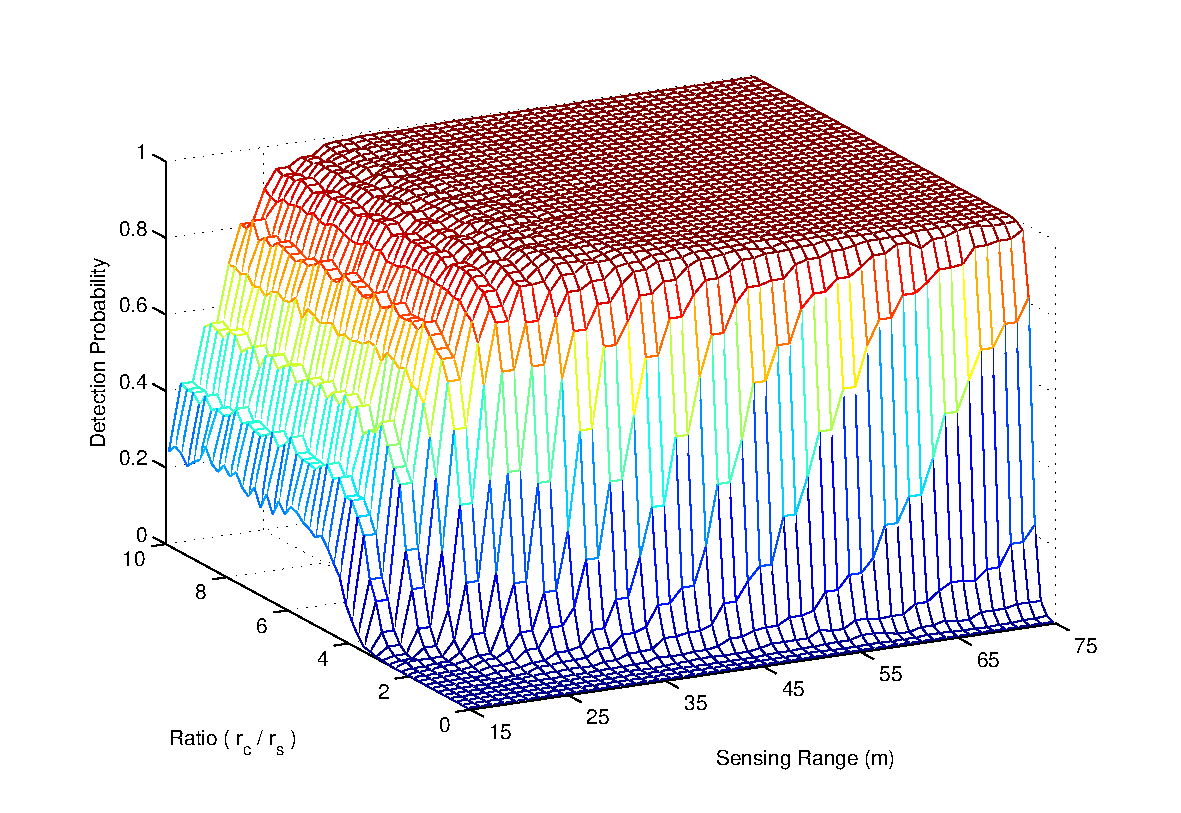
\includegraphics[width=3.2 in]{RandomKCover_DetectionProb_VariableRatio.eps}\\
  \caption{RandomKCover DetectionProb VariableRatio eps}\label{RandomKCover_DetectionProb_VariableRatio.eps}
\end{figure}


\begin{figure}
  % Requires \usepackage{graphicx}
  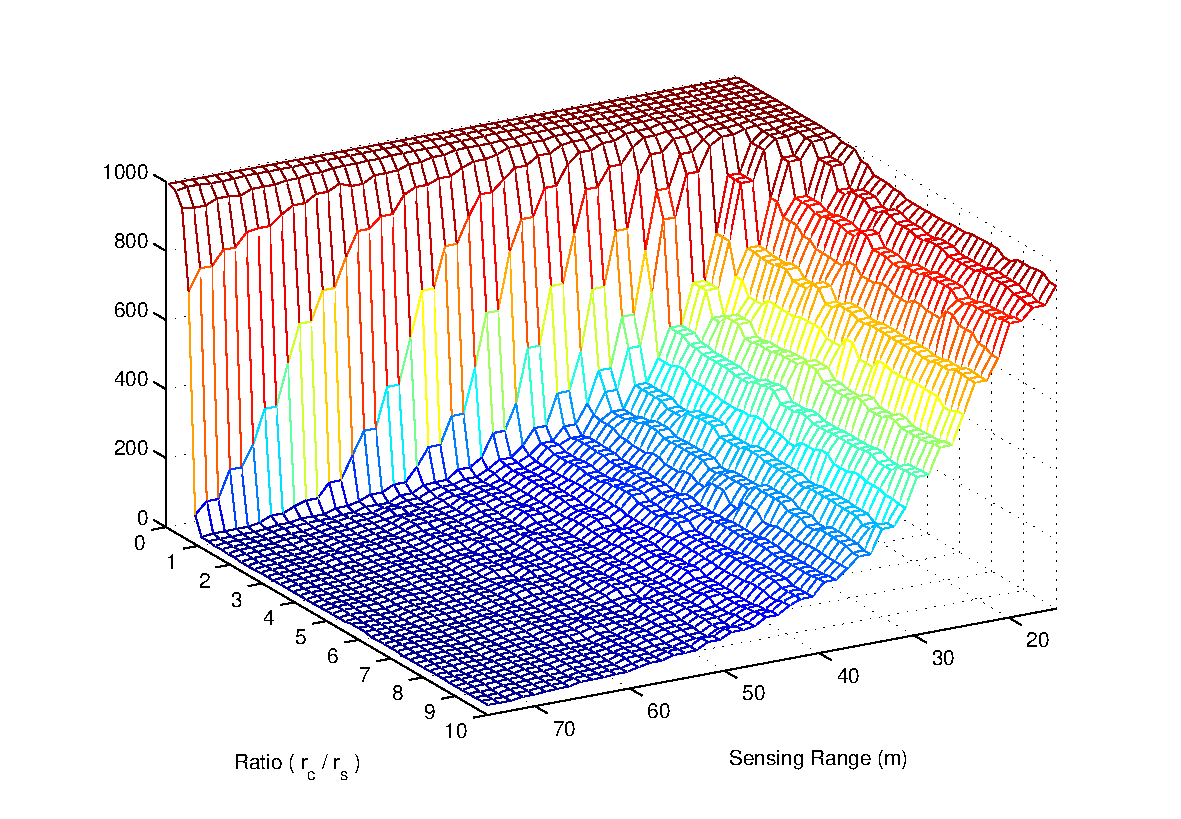
\includegraphics[width=3.2 in]{RandomKCover_DistanceTraveled_VariableRatio.eps}\\
  \caption{RandomKCover DistanceTraveled VariableRatio.eps}\label{RandomKCover_DistanceTraveled_VariableRatio.eps}
\end{figure}


\begin{figure}
  % Requires \usepackage{graphicx}
  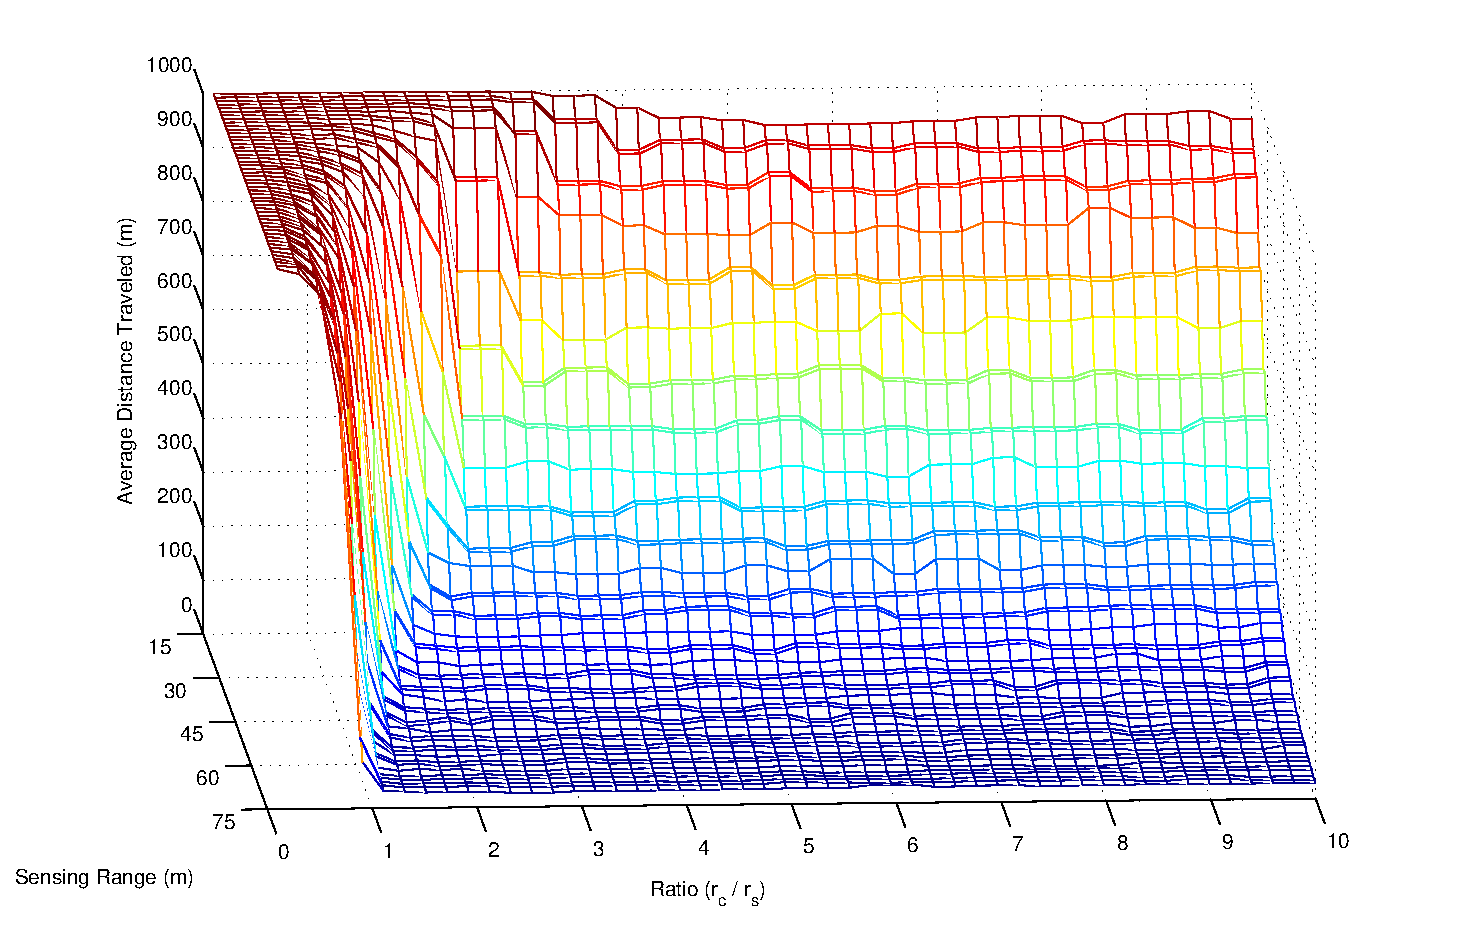
\includegraphics[width=3.2 in]{RandomKCover_DistanceTraveled_VariableRatio_v2.eps}\\
  \caption{RandomKCover DistanceTraveled VariableRatio v2.eps}\label{RandomKCover_DistanceTraveled_VariableRatio.eps}
\end{figure}





\section{Conclusion} \label{sec:conclusion}


\bibliographystyle{IEEEtran}
\bibliography{IEEEabrv,sensor}


\end{document}
